\documentclass[11pt,a4paper]{article}

% ============================================================================
% PACKAGES
% ============================================================================
\usepackage[utf8]{inputenc}
\usepackage[T1]{fontenc}
\usepackage{helvet}
\renewcommand{\familydefault}{\sfdefault}
\usepackage[margin=2.2cm, headheight=25pt]{geometry}
\usepackage{xcolor}
\usepackage{colortbl}
\usepackage{booktabs}
\usepackage{tabularx}
\usepackage{array}
\usepackage{graphicx}
\usepackage{tikz}
\usepackage{fancyhdr}
\usepackage{enumitem}
\usepackage{multirow}
\usepackage{pifont}
\usetikzlibrary{shapes.geometric, arrows, positioning, calc, patterns}

% ============================================================================
% COLOR DEFINITIONS
% ============================================================================
\definecolor{miloprimary}{RGB}{37, 99, 235}
\definecolor{milosecondary}{RGB}{99, 102, 241}
\definecolor{miloaccent}{RGB}{14, 165, 233}
\definecolor{freegray}{RGB}{107, 114, 128}
\definecolor{bronzecolor}{RGB}{205, 127, 50}
\definecolor{silvercolor}{RGB}{119, 136, 153}
\definecolor{goldcolor}{RGB}{212, 175, 55}
\definecolor{platinumcolor}{RGB}{139, 92, 246}
\definecolor{successgreen}{RGB}{34, 197, 94}
\definecolor{warningorange}{RGB}{249, 115, 22}
\definecolor{lightbg}{RGB}{248, 250, 252}
\definecolor{darktext}{RGB}{30, 41, 59}
\definecolor{darkgreen}{RGB}{22, 163, 74}

% ============================================================================
% HEADER/FOOTER CONFIGURATION
% ============================================================================
\pagestyle{fancy}
\fancyhf{}
\fancyhead[L]{\textcolor{miloprimary}{\textbf{MILO APP}}}
\fancyhead[R]{\textcolor{freegray}{Pricing Strategy v3.2}}
\fancyfoot[C]{\textcolor{freegray}{\thepage}}
\renewcommand{\headrulewidth}{2pt}
\renewcommand{\headrule}{\hbox to\headwidth{\color{miloprimary}\leaders\hrule height \headrulewidth\hfill}}

% ============================================================================
% CUSTOM COMMANDS
% ============================================================================
\newcommand{\tierbox}[5]{%
    \begin{tikzpicture}
        \node[fill=#1!12, draw=#1, line width=2pt, rounded corners=10pt,
              minimum width=3.5cm, minimum height=3.2cm, align=center] {
            \textcolor{#1}{\textbf{\large #2}}\\[6pt]
            \textcolor{darktext}{\textbf{#3} receipts}\\[4pt]
            \textcolor{#1}{\textbf{\Large #4}}\\[2pt]
            \textcolor{freegray}{\small #5}
        };
    \end{tikzpicture}%
}

\newcommand{\featurebox}[2]{%
    \begin{tikzpicture}
        \node[fill=#1!10, draw=#1, line width=1.5pt, rounded corners=8pt,
              inner sep=15pt, text width=\textwidth-35pt, align=left] {#2};
    \end{tikzpicture}%
}

\newcommand{\cmark}{\textcolor{successgreen}{\ding{51}}}

% ============================================================================
% DOCUMENT BEGIN
% ============================================================================
\begin{document}

% ============================================================================
% TITLE PAGE
% ============================================================================
\begin{center}
    \vspace*{0.3cm}
    {\Huge\textcolor{miloprimary}{\textbf{MILO APP}}}\\[0.4cm]
    {\LARGE\textcolor{milosecondary}{Tier-Based Pricing Strategy v3.2}}\\[0.2cm]
    {\large\textcolor{freegray}{Volume-Based Pricing with Full Feature Access}}\\[0.7cm]

    
\begin{tikzpicture}
        \node[fill=miloprimary!10, draw=miloprimary, line width=1.5pt, rounded corners=8pt,
              inner sep=12pt] {
            \textcolor{miloprimary}{\textbf{DeepmAInd B.V.} \quad|\quad Version 3.2 \quad|\quad January 2026}
        };
    \end{tikzpicture}
\end{center}

\vspace{0.6cm}

% ============================================================================
% PRICING MODEL OVERVIEW
% ============================================================================
\section*{\textcolor{miloprimary}{Pricing Model Overview}}

\begin{center}
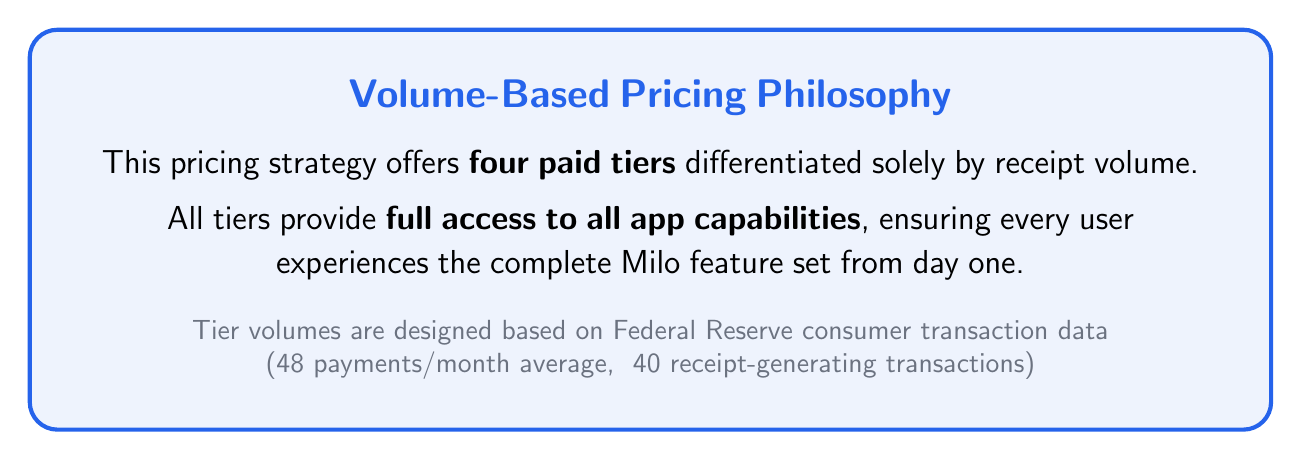
\begin{tikzpicture}
    \node[fill=miloprimary!8, draw=miloprimary, line width=1.5pt, rounded corners=10pt,
          inner sep=18pt, text width=14.5cm, align=center] {
        {\Large\textcolor{miloprimary}{\textbf{Volume-Based Pricing Philosophy}}}\\[12pt]
        {\large This pricing strategy offers \textbf{four paid tiers} differentiated solely by receipt volume.}\\[8pt]
        {\large All tiers provide \textbf{full access to all app capabilities}, ensuring every user}\\[4pt]
        {\large experiences the complete Milo feature set from day one.}\\[12pt]
        {\normalsize\textcolor{freegray}{Tier volumes are designed based on Federal Reserve consumer transaction data}}\\
        {\normalsize\textcolor{freegray}{(48 payments/month average, ~40 receipt-generating transactions)}}
    };
\end{tikzpicture}
\end{center}

\vspace{0.8cm}

% ============================================================================
% VISUAL TIER DISPLAY
% ============================================================================
\section*{\textcolor{miloprimary}{Pricing Tiers at a Glance}}

\begin{center}
    \tierbox{freegray}{FREE TRIAL}{15}{\$0}{14 days}
    \hspace{0.3cm}
    \tierbox{bronzecolor}{BRONZE}{20}{\$2/mo}{\$20/year}
    \hspace{0.3cm}
    \tierbox{silvercolor}{SILVER}{40}{\$4/mo}{\$40/year}
    \hspace{0.3cm}
    \tierbox{goldcolor}{GOLD}{60}{\$6/mo}{\$60/year}
    \hspace{0.3cm}
    \tierbox{platinumcolor}{PLATINUM}{100}{\$10/mo}{\$100/year}
\end{center}

\vspace{0.8cm}

% ============================================================================
% PRICING TABLE
% ============================================================================
\section*{\textcolor{miloprimary}{Detailed Pricing Structure}}

\begin{center}
\renewcommand{\arraystretch}{1.7}
\begin{tabular}{>{\centering\arraybackslash}p{2.5cm} >{\centering\arraybackslash}p{2.2cm} >{\centering\arraybackslash}p{2.2cm} >{\centering\arraybackslash}p{2.2cm} >{\centering\arraybackslash}p{2.5cm} >{\centering\arraybackslash}p{2.5cm}}
\toprule
\rowcolor{miloprimary!15}
\textbf{Tier} & \textbf{Receipts/Mo} & \textbf{Monthly} & \textbf{Annual} & \textbf{Per Receipt} & \textbf{Features} \\
\midrule
\rowcolor{freegray!8}
\textcolor{freegray}{\textbf{Free Trial}} & 15 total & Free & -- & -- & \cellcolor{successgreen!15}\textcolor{successgreen}{\textbf{Full Access}} \\
\rowcolor{bronzecolor!8}
\textcolor{bronzecolor}{\textbf{Bronze}} & 20 & \$2 & \$20 & \$0.10 & \cellcolor{successgreen!15}\textcolor{successgreen}{\textbf{Full Access}} \\
\rowcolor{silvercolor!8}
\textcolor{silvercolor}{\textbf{Silver}} & 40 & \$4 & \$40 & \$0.10 & \cellcolor{successgreen!15}\textcolor{successgreen}{\textbf{Full Access}} \\
\rowcolor{goldcolor!8}
\textcolor{goldcolor}{\textbf{Gold}} & 60 & \$6 & \$60 & \$0.10 & \cellcolor{successgreen!15}\textcolor{successgreen}{\textbf{Full Access}} \\
\rowcolor{platinumcolor!8}
\textcolor{platinumcolor}{\textbf{Platinum}} & 100 & \$10 & \$100 & \$0.10 & \cellcolor{successgreen!15}\textcolor{successgreen}{\textbf{Full Access}} \\
\bottomrule
\end{tabular}
\end{center}

\vspace{0.3cm}

\begin{center}

\begin{tikzpicture}
    \node[fill=successgreen!10, draw=successgreen, line width=1pt, rounded corners=5pt,
          inner sep=10pt, text width=14cm, align=center] {
        \textcolor{darkgreen}{\textbf{Annual Savings:}} All annual plans offer \textbf{17\% discount} compared to monthly billing
    };
\end{tikzpicture}
\end{center}

\newpage

% ============================================================================
% TIER DETAILS
% ============================================================================
\section*{\textcolor{miloprimary}{Tier Details \& Target Users}}

% Free Trial
\subsection*{\textcolor{freegray}{Free Trial}}

\begin{center}
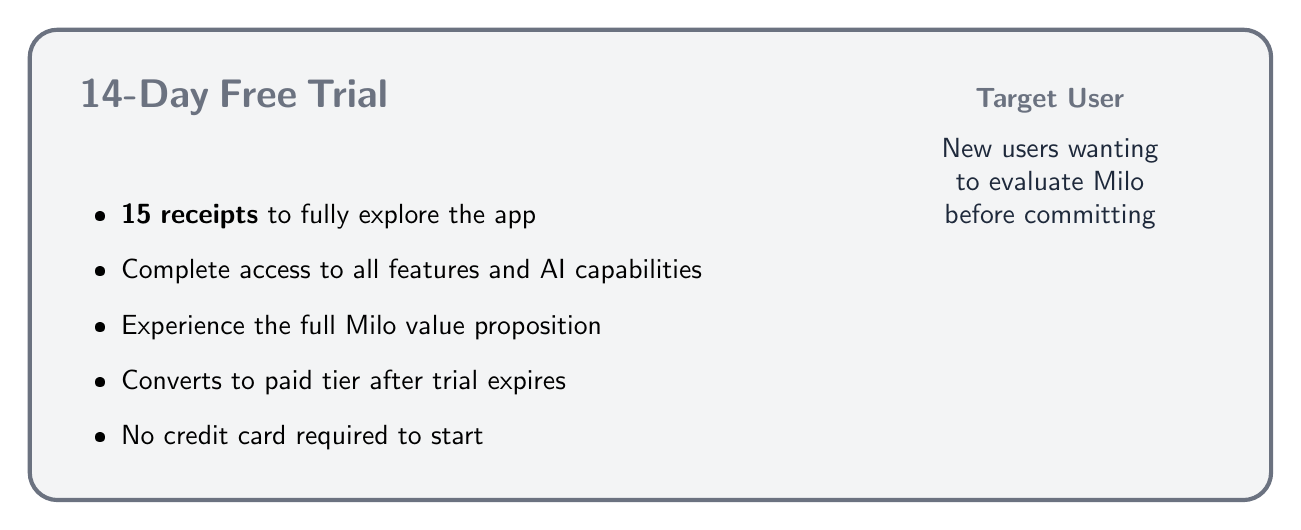
\begin{tikzpicture}
    \node[fill=freegray!8, draw=freegray, line width=1.5pt, rounded corners=10pt,
          inner sep=18pt, text width=14.5cm, align=left] {
        \begin{minipage}[t]{0.65\textwidth}
            \textcolor{freegray}{\textbf{\Large 14-Day Free Trial}}\\[10pt]
            \begin{itemize}[leftmargin=1.5em, itemsep=4pt]
                \item \textbf{15 receipts} to fully explore the app
                \item Complete access to all features and AI capabilities
                \item Experience the full Milo value proposition
                \item Converts to paid tier after trial expires
                \item No credit card required to start
            \end{itemize}
        \end{minipage}
        \hfill
        \begin{minipage}[t]{0.30\textwidth}
            \begin{center}
                \textcolor{freegray}{\textbf{Target User}}\\[6pt]
                \textcolor{darktext}{New users wanting\\to evaluate Milo\\before committing}
            \end{center}
        \end{minipage}
    };
\end{tikzpicture}
\end{center}

\vspace{0.5cm}

% Bronze
\subsection*{\textcolor{bronzecolor}{Bronze}}

\begin{center}
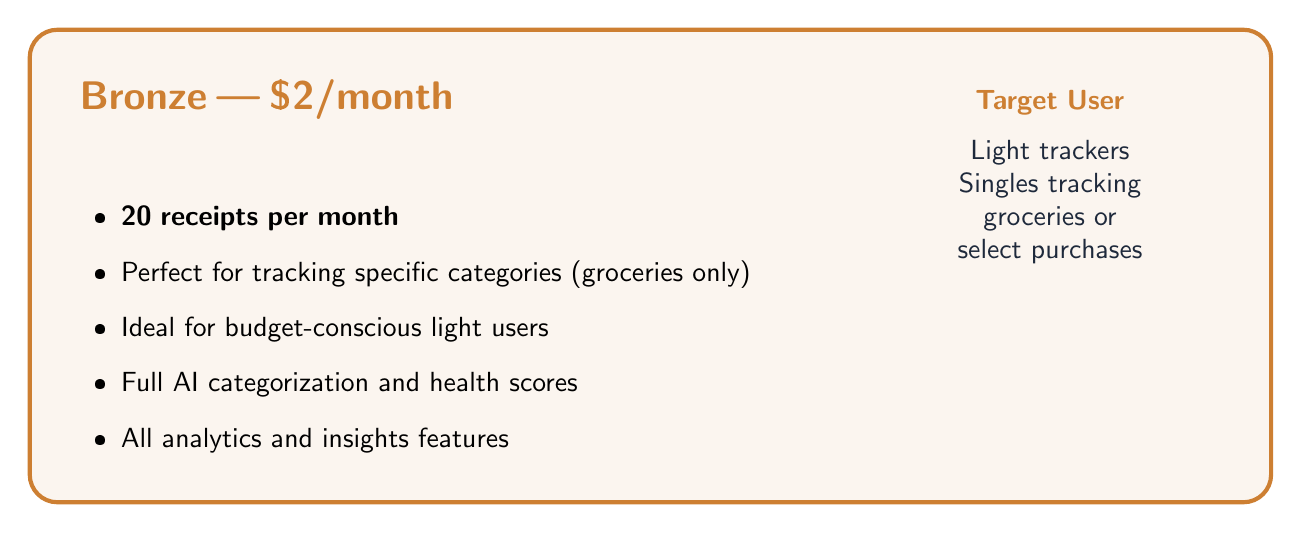
\begin{tikzpicture}
    \node[fill=bronzecolor!8, draw=bronzecolor, line width=1.5pt, rounded corners=10pt,
          inner sep=18pt, text width=14.5cm, align=left] {
        \begin{minipage}[t]{0.65\textwidth}
            \textcolor{bronzecolor}{\textbf{\Large Bronze --- \$2/month}}\\[10pt]
            \begin{itemize}[leftmargin=1.5em, itemsep=4pt]
                \item \textbf{20 receipts per month}
                \item Perfect for tracking specific categories (groceries only)
                \item Ideal for budget-conscious light users
                \item Full AI categorization and health scores
                \item All analytics and insights features
            \end{itemize}
        \end{minipage}
        \hfill
        \begin{minipage}[t]{0.30\textwidth}
            \begin{center}
                \textcolor{bronzecolor}{\textbf{Target User}}\\[6pt]
                \textcolor{darktext}{Light trackers\\Singles tracking\\groceries or\\select purchases}
            \end{center}
        \end{minipage}
    };
\end{tikzpicture}
\end{center}

\vspace{0.5cm}

% Silver
\subsection*{\textcolor{silvercolor}{Silver}}

\begin{center}
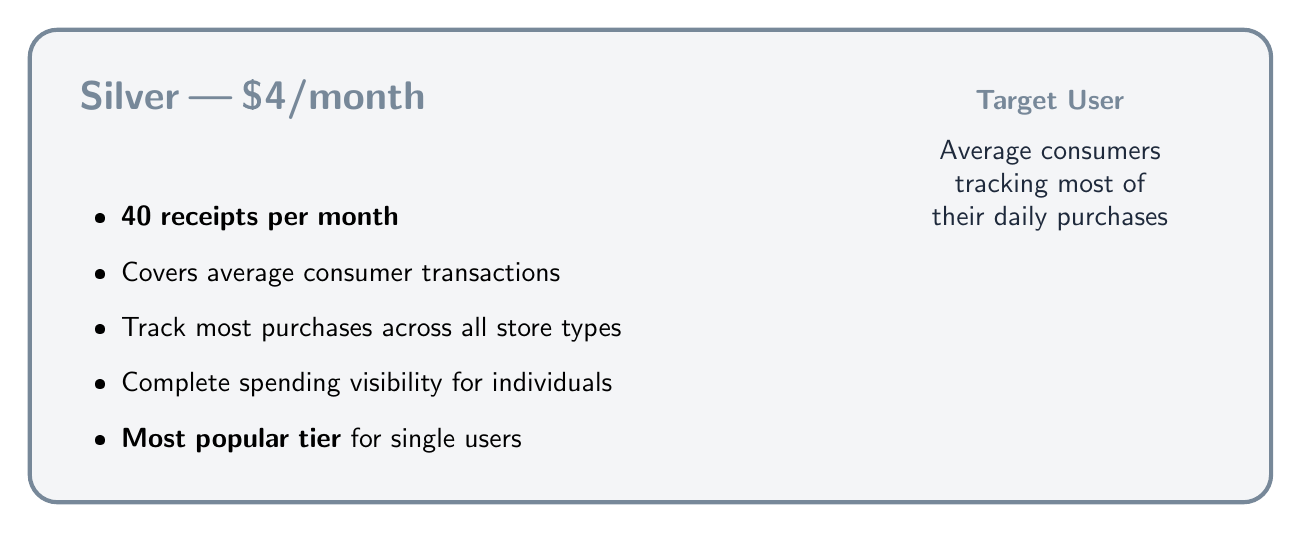
\begin{tikzpicture}
    \node[fill=silvercolor!8, draw=silvercolor, line width=1.5pt, rounded corners=10pt,
          inner sep=18pt, text width=14.5cm, align=left] {
        \begin{minipage}[t]{0.65\textwidth}
            \textcolor{silvercolor}{\textbf{\Large Silver --- \$4/month}}\\[10pt]
            \begin{itemize}[leftmargin=1.5em, itemsep=4pt]
                \item \textbf{40 receipts per month}
                \item Covers average consumer transactions
                \item Track most purchases across all store types
                \item Complete spending visibility for individuals
                \item \textbf{Most popular tier} for single users
            \end{itemize}
        \end{minipage}
        \hfill
        \begin{minipage}[t]{0.30\textwidth}
            \begin{center}
                \textcolor{silvercolor}{\textbf{Target User}}\\[6pt]
                \textcolor{darktext}{Average consumers\\tracking most of\\their daily purchases}
            \end{center}
        \end{minipage}
    };
\end{tikzpicture}
\end{center}

\newpage

% Gold
\subsection*{\textcolor{goldcolor}{Gold}}

\begin{center}
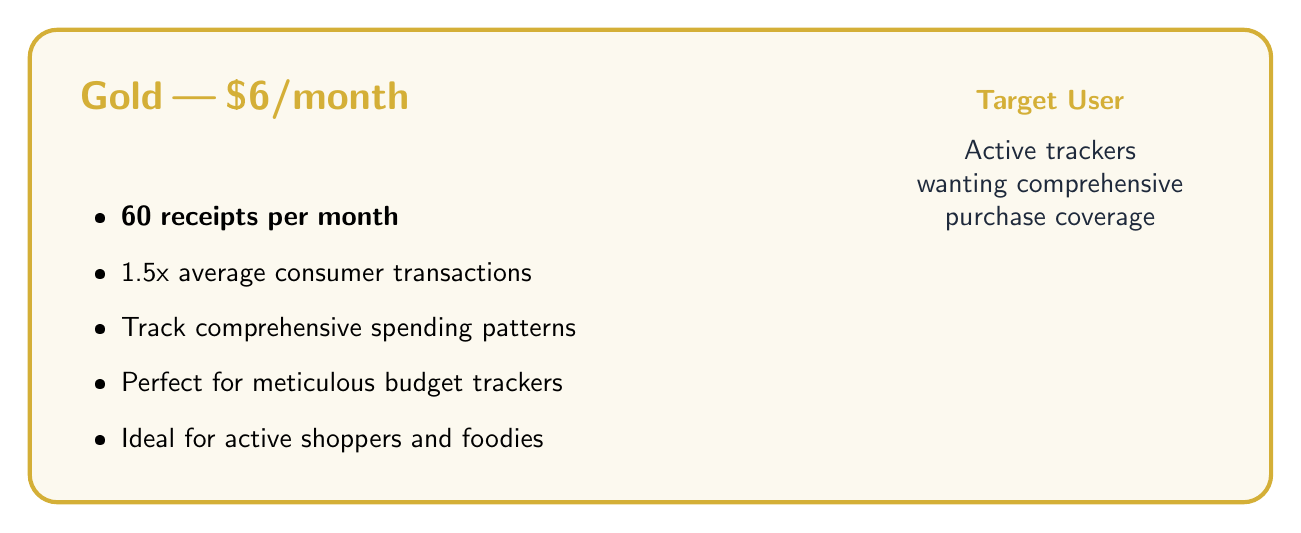
\begin{tikzpicture}
    \node[fill=goldcolor!8, draw=goldcolor, line width=1.5pt, rounded corners=10pt,
          inner sep=18pt, text width=14.5cm, align=left] {
        \begin{minipage}[t]{0.65\textwidth}
            \textcolor{goldcolor}{\textbf{\Large Gold --- \$6/month}}\\[10pt]
            \begin{itemize}[leftmargin=1.5em, itemsep=4pt]
                \item \textbf{60 receipts per month}
                \item 1.5x average consumer transactions
                \item Track comprehensive spending patterns
                \item Perfect for meticulous budget trackers
                \item Ideal for active shoppers and foodies
            \end{itemize}
        \end{minipage}
        \hfill
        \begin{minipage}[t]{0.30\textwidth}
            \begin{center}
                \textcolor{goldcolor}{\textbf{Target User}}\\[6pt]
                \textcolor{darktext}{Active trackers\\wanting comprehensive\\purchase coverage}
            \end{center}
        \end{minipage}
    };
\end{tikzpicture}
\end{center}

\vspace{0.5cm}

% Platinum
\subsection*{\textcolor{platinumcolor}{Platinum}}

\begin{center}
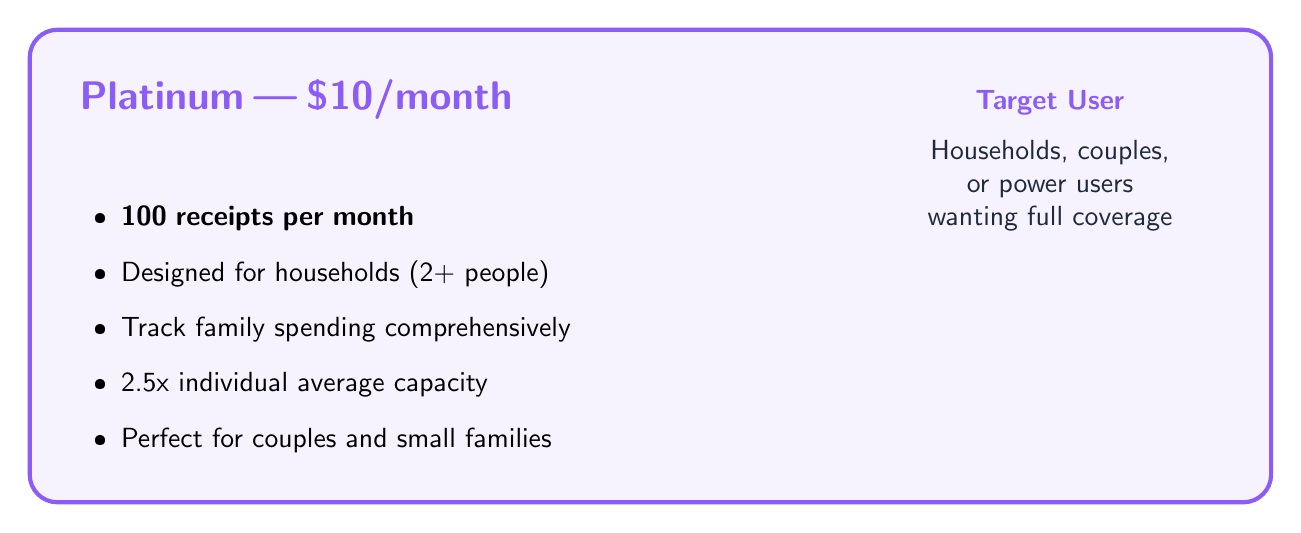
\begin{tikzpicture}
    \node[fill=platinumcolor!8, draw=platinumcolor, line width=1.5pt, rounded corners=10pt,
          inner sep=18pt, text width=14.5cm, align=left] {
        \begin{minipage}[t]{0.65\textwidth}
            \textcolor{platinumcolor}{\textbf{\Large Platinum --- \$10/month}}\\[10pt]
            \begin{itemize}[leftmargin=1.5em, itemsep=4pt]
                \item \textbf{100 receipts per month}
                \item Designed for households (2+ people)
                \item Track family spending comprehensively
                \item 2.5x individual average capacity
                \item Perfect for couples and small families
            \end{itemize}
        \end{minipage}
        \hfill
        \begin{minipage}[t]{0.30\textwidth}
            \begin{center}
                \textcolor{platinumcolor}{\textbf{Target User}}\\[6pt]
                \textcolor{darktext}{Households, couples,\\or power users\\wanting full coverage}
            \end{center}
        \end{minipage}
    };
\end{tikzpicture}
\end{center}

\vspace{0.8cm}

% ============================================================================
% FEATURES INCLUDED
% ============================================================================
\section*{\textcolor{miloprimary}{Features Included in All Tiers}}

\begin{center}
\featurebox{successgreen}{
    \textcolor{darkgreen}{\textbf{\Large Full Feature Access --- Every Tier}}\\[12pt]
    \begin{minipage}[t]{0.48\textwidth}
        \textbf{Core Features}
        \begin{itemize}[leftmargin=1.5em, itemsep=3pt]
            \item[\cmark] Receipt scanning \& OCR extraction
            \item[\cmark] AI-powered categorization
            \item[\cmark] Health scores (0--5 scale)
            \item[\cmark] 16 spending categories
            \item[\cmark] AI chat assistant
        \end{itemize}
    \end{minipage}
    \hfill
    \begin{minipage}[t]{0.48\textwidth}
        \textbf{Analytics \& Insights}
        \begin{itemize}[leftmargin=1.5em, itemsep=3pt]
            \item[\cmark] Spending analytics dashboard
            \item[\cmark] Monthly spending summaries
            \item[\cmark] Store price comparisons
            \item[\cmark] Trend analysis over time
            \item[\cmark] Data export (CSV, PDF)
        \end{itemize}
    \end{minipage}
}
\end{center}

\newpage

% ============================================================================
% RESEARCH BASIS
% ============================================================================
\section*{\textcolor{miloprimary}{Research-Based Tier Design}}

\begin{center}
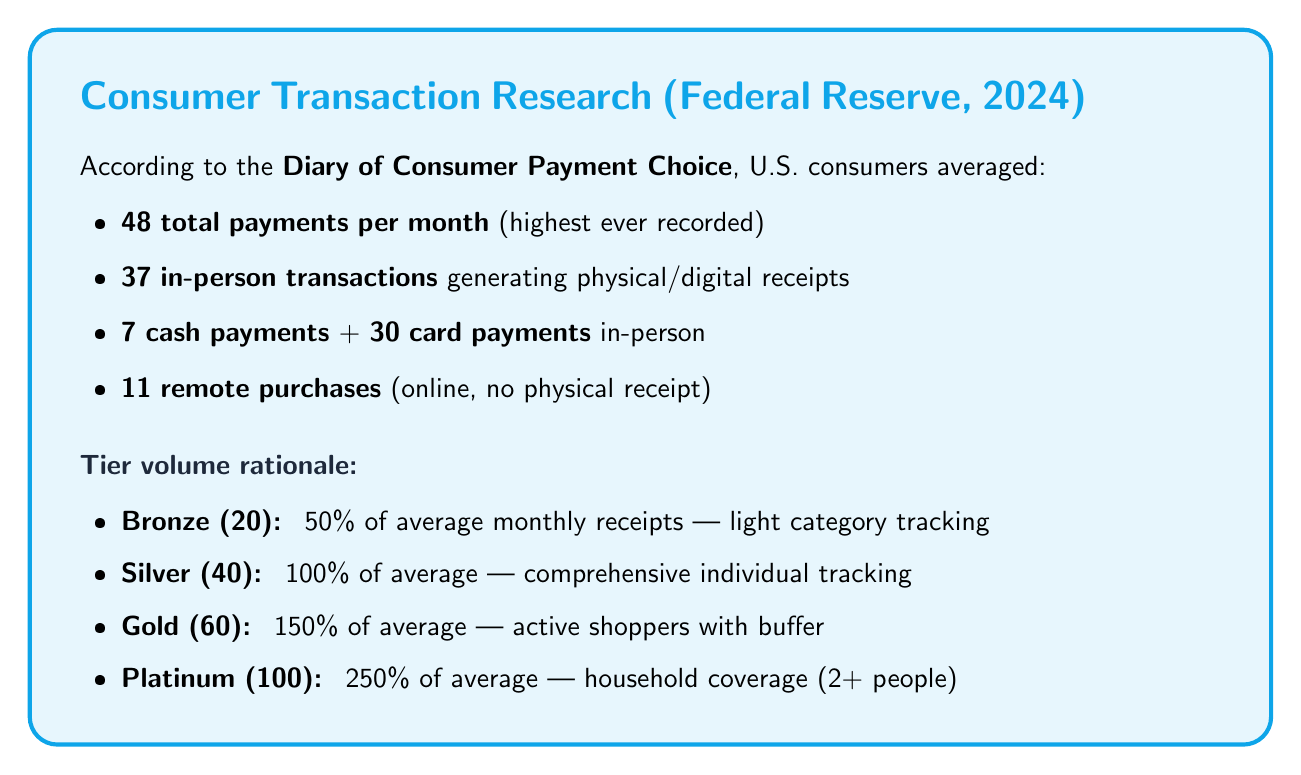
\begin{tikzpicture}
    \node[fill=miloaccent!10, draw=miloaccent, line width=1.5pt, rounded corners=10pt,
          inner sep=18pt, text width=14.5cm, align=left] {
        \textcolor{miloaccent}{\textbf{\Large Consumer Transaction Research (Federal Reserve, 2024)}}\\[12pt]
        According to the \textbf{Diary of Consumer Payment Choice}, U.S. consumers averaged:
        \begin{itemize}[leftmargin=1.5em, itemsep=4pt]
            \item \textbf{48 total payments per month} (highest ever recorded)
            \item \textbf{37 in-person transactions} generating physical/digital receipts
            \item \textbf{7 cash payments} + \textbf{30 card payments} in-person
            \item \textbf{11 remote purchases} (online, no physical receipt)
        \end{itemize}
        \vspace{8pt}
        \textcolor{darktext}{\textbf{Tier volume rationale:}}
        \begin{itemize}[leftmargin=1.5em, itemsep=3pt]
            \item \textbf{Bronze (20):} ~50\% of average monthly receipts --- light category tracking
            \item \textbf{Silver (40):} ~100\% of average --- comprehensive individual tracking
            \item \textbf{Gold (60):} ~150\% of average --- active shoppers with buffer
            \item \textbf{Platinum (100):} ~250\% of average --- household coverage (2+ people)
        \end{itemize}
    };
\end{tikzpicture}
\end{center}

\vspace{0.6cm}

% ============================================================================
% ANNUAL SAVINGS
% ============================================================================
\section*{\textcolor{miloprimary}{Annual Subscription Savings}}

\begin{center}
\renewcommand{\arraystretch}{1.6}
\begin{tabular}{>{\centering\arraybackslash}p{3cm} >{\centering\arraybackslash}p{3cm} >{\centering\arraybackslash}p{3cm} >{\centering\arraybackslash}p{3cm}}
\toprule
\rowcolor{miloprimary!15}
\textbf{Tier} & \textbf{Monthly Total} & \textbf{Annual Price} & \textbf{You Save} \\
\midrule
\rowcolor{bronzecolor!8}
\textcolor{bronzecolor}{\textbf{Bronze}} & \$24/year & \$20/year & \textcolor{darkgreen}{\textbf{\$4 (17\%)}} \\
\rowcolor{silvercolor!8}
\textcolor{silvercolor}{\textbf{Silver}} & \$48/year & \$40/year & \textcolor{darkgreen}{\textbf{\$8 (17\%)}} \\
\rowcolor{goldcolor!8}
\textcolor{goldcolor}{\textbf{Gold}} & \$72/year & \$60/year & \textcolor{darkgreen}{\textbf{\$12 (17\%)}} \\
\rowcolor{platinumcolor!8}
\textcolor{platinumcolor}{\textbf{Platinum}} & \$120/year & \$100/year & \textcolor{darkgreen}{\textbf{\$20 (17\%)}} \\
\bottomrule
\end{tabular}
\end{center}

\vspace{0.6cm}

\begin{center}

\begin{tikzpicture}
    \node[fill=successgreen!10, draw=successgreen, line width=1.5pt, rounded corners=8pt,
          inner sep=15pt, text width=14cm, align=center] {
        \textcolor{darkgreen}{\textbf{Annual billing is encouraged}}\\[6pt]
        \textcolor{darktext}{17\% savings + better retention + predictable revenue}
    };
\end{tikzpicture}
\end{center}

\newpage

% ============================================================================
% COMPETITIVE POSITIONING
% ============================================================================
\section*{\textcolor{miloprimary}{Competitive Positioning}}

\begin{center}
\renewcommand{\arraystretch}{1.5}
\begin{tabular}{>{\raggedright\arraybackslash}p{3.5cm} >{\centering\arraybackslash}p{2.5cm} >{\centering\arraybackslash}p{2.5cm} >{\centering\arraybackslash}p{2.5cm} >{\centering\arraybackslash}p{2.5cm}}
\toprule
\rowcolor{miloprimary!15}
\textbf{Feature} & \textbf{Milo} & \textbf{Competitor A} & \textbf{Competitor B} & \textbf{Competitor C} \\
\midrule
Entry Price & \textcolor{successgreen}{\textbf{\$2/mo}} & \$5/mo & \$4/mo & Free* \\
\rowcolor{lightbg}
AI Categorization & \cmark & \cmark & -- & -- \\
Health Scores & \cmark & -- & -- & -- \\
\rowcolor{lightbg}
Top Tier & \textcolor{successgreen}{\textbf{\$10/mo}} & \$25/mo & \$15/mo & \$10/mo* \\
Full Features All Tiers & \cmark & -- & -- & -- \\
\rowcolor{lightbg}
AI Chat Assistant & \cmark & -- & \cmark & -- \\
\bottomrule
\end{tabular}
\end{center}

{\small *Limited functionality or ad-supported}

\vspace{0.6cm}

% ============================================================================
% VALUE PROPOSITION
% ============================================================================
\section*{\textcolor{miloprimary}{Key Differentiators}}

\begin{center}
\begin{tikzpicture}
    \node[fill=miloprimary!8, draw=miloprimary, line width=2pt, rounded corners=12pt,
          inner sep=20pt, text width=14.5cm, align=center] {
        {\Large\textcolor{miloprimary}{\textbf{Volume-Based Pricing}}}\\[15pt]
        {\large All tiers include the \textbf{complete Milo experience}.}\\[10pt]
        {\large Choose your tier based solely on \textbf{how many receipts} you scan per month.}\\[10pt]
        {\large\textbf{No feature limitations. No upsell walls. No hidden costs.}}\\[15pt]
        \begin{tikzpicture}
            \node[fill=successgreen!15, draw=successgreen, line width=1pt, rounded corners=5pt,
                  inner sep=8pt] {
                \textcolor{darkgreen}{\textbf{Simple, transparent, fair pricing}}
            };
        \end{tikzpicture}
    };
\end{tikzpicture}
\end{center}

\vspace{0.8cm}

% ============================================================================
% UPGRADE PATH
% ============================================================================
\section*{\textcolor{miloprimary}{Seamless Upgrade Path}}

\begin{center}

\begin{tikzpicture}[node distance=1.5cm]
    % Nodes
    \node[fill=freegray!15, draw=freegray, line width=1pt, rounded corners=5pt,
          minimum width=2.5cm, minimum height=1.2cm, align=center] (trial) {\textbf{Free Trial}\\15 receipts};

    \node[fill=bronzecolor!15, draw=bronzecolor, line width=1pt, rounded corners=5pt,
          minimum width=2.5cm, minimum height=1.2cm, align=center, right=of trial] (bronze) {\textbf{Bronze}\\20/mo};

    \node[fill=silvercolor!15, draw=silvercolor, line width=1pt, rounded corners=5pt,
          minimum width=2.5cm, minimum height=1.2cm, align=center, right=of bronze] (silver) {\textbf{Silver}\\40/mo};

    \node[fill=goldcolor!15, draw=goldcolor, line width=1pt, rounded corners=5pt,
          minimum width=2.5cm, minimum height=1.2cm, align=center, right=of silver] (gold) {\textbf{Gold}\\60/mo};

    \node[fill=platinumcolor!15, draw=platinumcolor, line width=1pt, rounded corners=5pt,
          minimum width=2.5cm, minimum height=1.2cm, align=center, right=of gold] (platinum) {\textbf{Platinum}\\100/mo};

    % Arrows
    \draw[->, line width=1.5pt, miloprimary] (trial) -- (bronze);
    \draw[->, line width=1.5pt, miloprimary] (bronze) -- (silver);
    \draw[->, line width=1.5pt, miloprimary] (silver) -- (gold);
    \draw[->, line width=1.5pt, miloprimary] (gold) -- (platinum);
\end{tikzpicture}
\end{center}

\vspace{0.3cm}

\begin{center}

\begin{tikzpicture}
    \node[fill=lightbg, draw=freegray, line width=1pt, rounded corners=5pt,
          inner sep=12pt, text width=14cm, align=center] {
        \textcolor{freegray}{\textbf{Users can upgrade or downgrade anytime.}\\
        Pro-rated billing ensures fair charges. No lock-in contracts.}
    };
\end{tikzpicture}
\end{center}

\newpage

% ============================================================================
% BUSINESS RATIONALE
% ============================================================================
\section*{\textcolor{miloprimary}{Business Rationale}}

\begin{center}
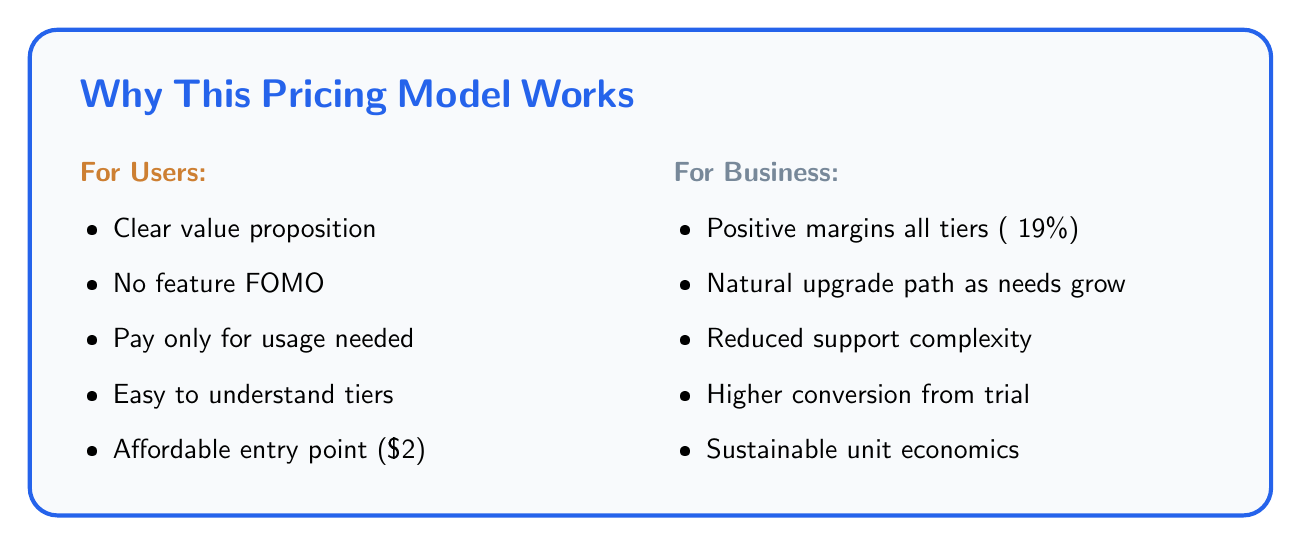
\begin{tikzpicture}
    \node[fill=lightbg, draw=miloprimary, line width=1.5pt, rounded corners=10pt,
          inner sep=18pt, text width=14.5cm, align=left] {
        \textcolor{miloprimary}{\textbf{\Large Why This Pricing Model Works}}\\[15pt]

        \begin{minipage}[t]{0.48\textwidth}
            \textbf{\textcolor{bronzecolor}{For Users:}}
            \begin{itemize}[leftmargin=1.2em, itemsep=4pt]
                \item Clear value proposition
                \item No feature FOMO
                \item Pay only for usage needed
                \item Easy to understand tiers
                \item Affordable entry point (\$2)
            \end{itemize}
        \end{minipage}
        \hfill
        \begin{minipage}[t]{0.48\textwidth}
            \textbf{\textcolor{silvercolor}{For Business:}}
            \begin{itemize}[leftmargin=1.2em, itemsep=4pt]
                \item Positive margins all tiers (~19\%)
                \item Natural upgrade path as needs grow
                \item Reduced support complexity
                \item Higher conversion from trial
                \item Sustainable unit economics
            \end{itemize}
        \end{minipage}
    };
\end{tikzpicture}
\end{center}

\vspace{0.6cm}

% ============================================================================
% MARGIN SUMMARY
% ============================================================================
\section*{\textcolor{miloprimary}{Unit Economics Summary}}

\begin{center}
\renewcommand{\arraystretch}{1.5}
\begin{tabular}{>{\centering\arraybackslash}p{2.5cm} >{\centering\arraybackslash}p{2cm} >{\centering\arraybackslash}p{2.5cm} >{\centering\arraybackslash}p{2.5cm} >{\centering\arraybackslash}p{2.5cm}}
\toprule
\rowcolor{miloprimary!15}
\textbf{Tier} & \textbf{Price} & \textbf{Variable Cost} & \textbf{Gross Profit} & \textbf{Gross Margin} \\
\midrule
\rowcolor{bronzecolor!8}
\textcolor{bronzecolor}{\textbf{Bronze}} & \$2.00 & \$1.63 & \$0.37 & \textcolor{darkgreen}{\textbf{18.5\%}} \\
\rowcolor{silvercolor!8}
\textcolor{silvercolor}{\textbf{Silver}} & \$4.00 & \$3.24 & \$0.76 & \textcolor{darkgreen}{\textbf{19.0\%}} \\
\rowcolor{goldcolor!8}
\textcolor{goldcolor}{\textbf{Gold}} & \$6.00 & \$4.87 & \$1.13 & \textcolor{darkgreen}{\textbf{18.8\%}} \\
\rowcolor{platinumcolor!8}
\textcolor{platinumcolor}{\textbf{Platinum}} & \$10.00 & \$8.10 & \$1.90 & \textcolor{darkgreen}{\textbf{19.0\%}} \\
\bottomrule
\end{tabular}
\end{center}

\vspace{0.3cm}

\begin{center}

\begin{tikzpicture}
    \node[fill=successgreen!10, draw=successgreen, line width=1.5pt, rounded corners=8pt,
          inner sep=12pt, text width=14cm, align=center] {
        \textcolor{darkgreen}{\textbf{All paid tiers achieve consistent ~19\% gross margins}}\\[4pt]
        \textcolor{darktext}{Sustainable pricing that balances user value with business viability}
    };
\end{tikzpicture}
\end{center}

\vspace{0.8cm}

% ============================================================================
% PRICING PSYCHOLOGY
% ============================================================================
\section*{\textcolor{miloprimary}{Pricing Psychology}}

\begin{center}
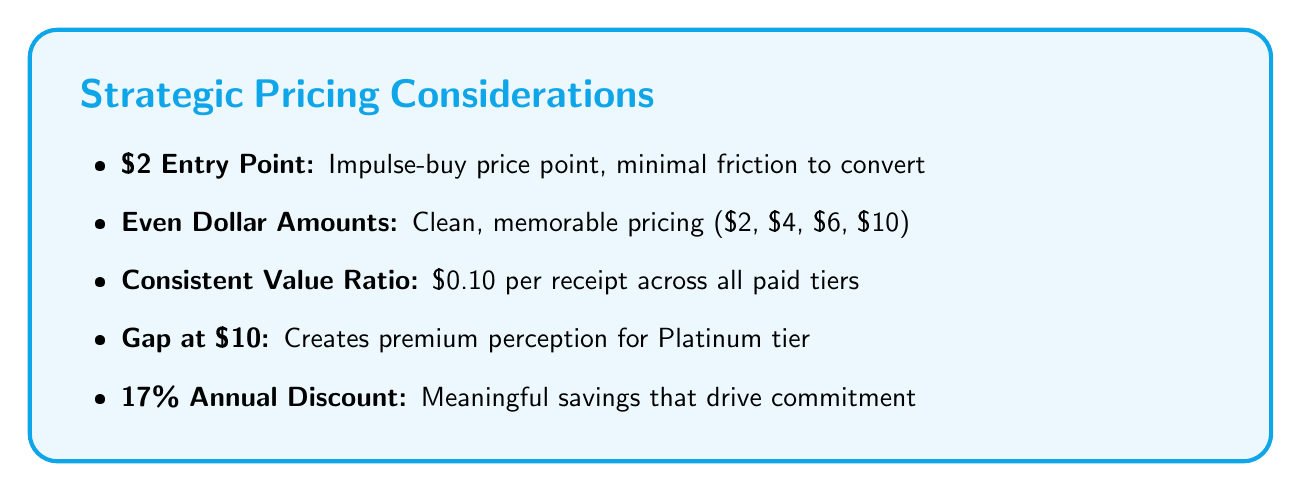
\begin{tikzpicture}
    \node[fill=miloaccent!8, draw=miloaccent, line width=1.5pt, rounded corners=10pt,
          inner sep=18pt, text width=14.5cm, align=left] {
        \textcolor{miloaccent}{\textbf{\Large Strategic Pricing Considerations}}\\[12pt]
        \begin{itemize}[leftmargin=1.5em, itemsep=5pt]
            \item \textbf{\$2 Entry Point:} Impulse-buy price point, minimal friction to convert
            \item \textbf{Even Dollar Amounts:} Clean, memorable pricing (\$2, \$4, \$6, \$10)
            \item \textbf{Consistent Value Ratio:} \$0.10 per receipt across all paid tiers
            \item \textbf{Gap at \$10:} Creates premium perception for Platinum tier
            \item \textbf{17\% Annual Discount:} Meaningful savings that drive commitment
        \end{itemize}
    };
\end{tikzpicture}
\end{center}

\vspace{1cm}

% ============================================================================
% FOOTER
% ============================================================================
\begin{center}
    \textcolor{freegray}{\rule{14cm}{0.5pt}}\\[0.4cm]
    \textcolor{freegray}{\small DeepmAInd B.V. | Confidential | Version 3.2 | January 2026}\\[0.2cm]
    \textcolor{freegray}{\scriptsize Research basis: Federal Reserve Diary of Consumer Payment Choice (2024)}
\end{center}

\end{document}
